\section{Laborversuch Ernährung des Pantoffeltierchens}
Pantoffeltierchen werden mit eingefärbter Hefe gefüttert. 
Dabei soll die Aufnahme der Hefe durch das Pantoffeltierchen und die 
anschliessende Verdauung beobachtet werden. Die Verdauung ist als Farbänderung 
rot $\to$ blau erkennbar. 
\begin{figure}[h!]
    \centering
    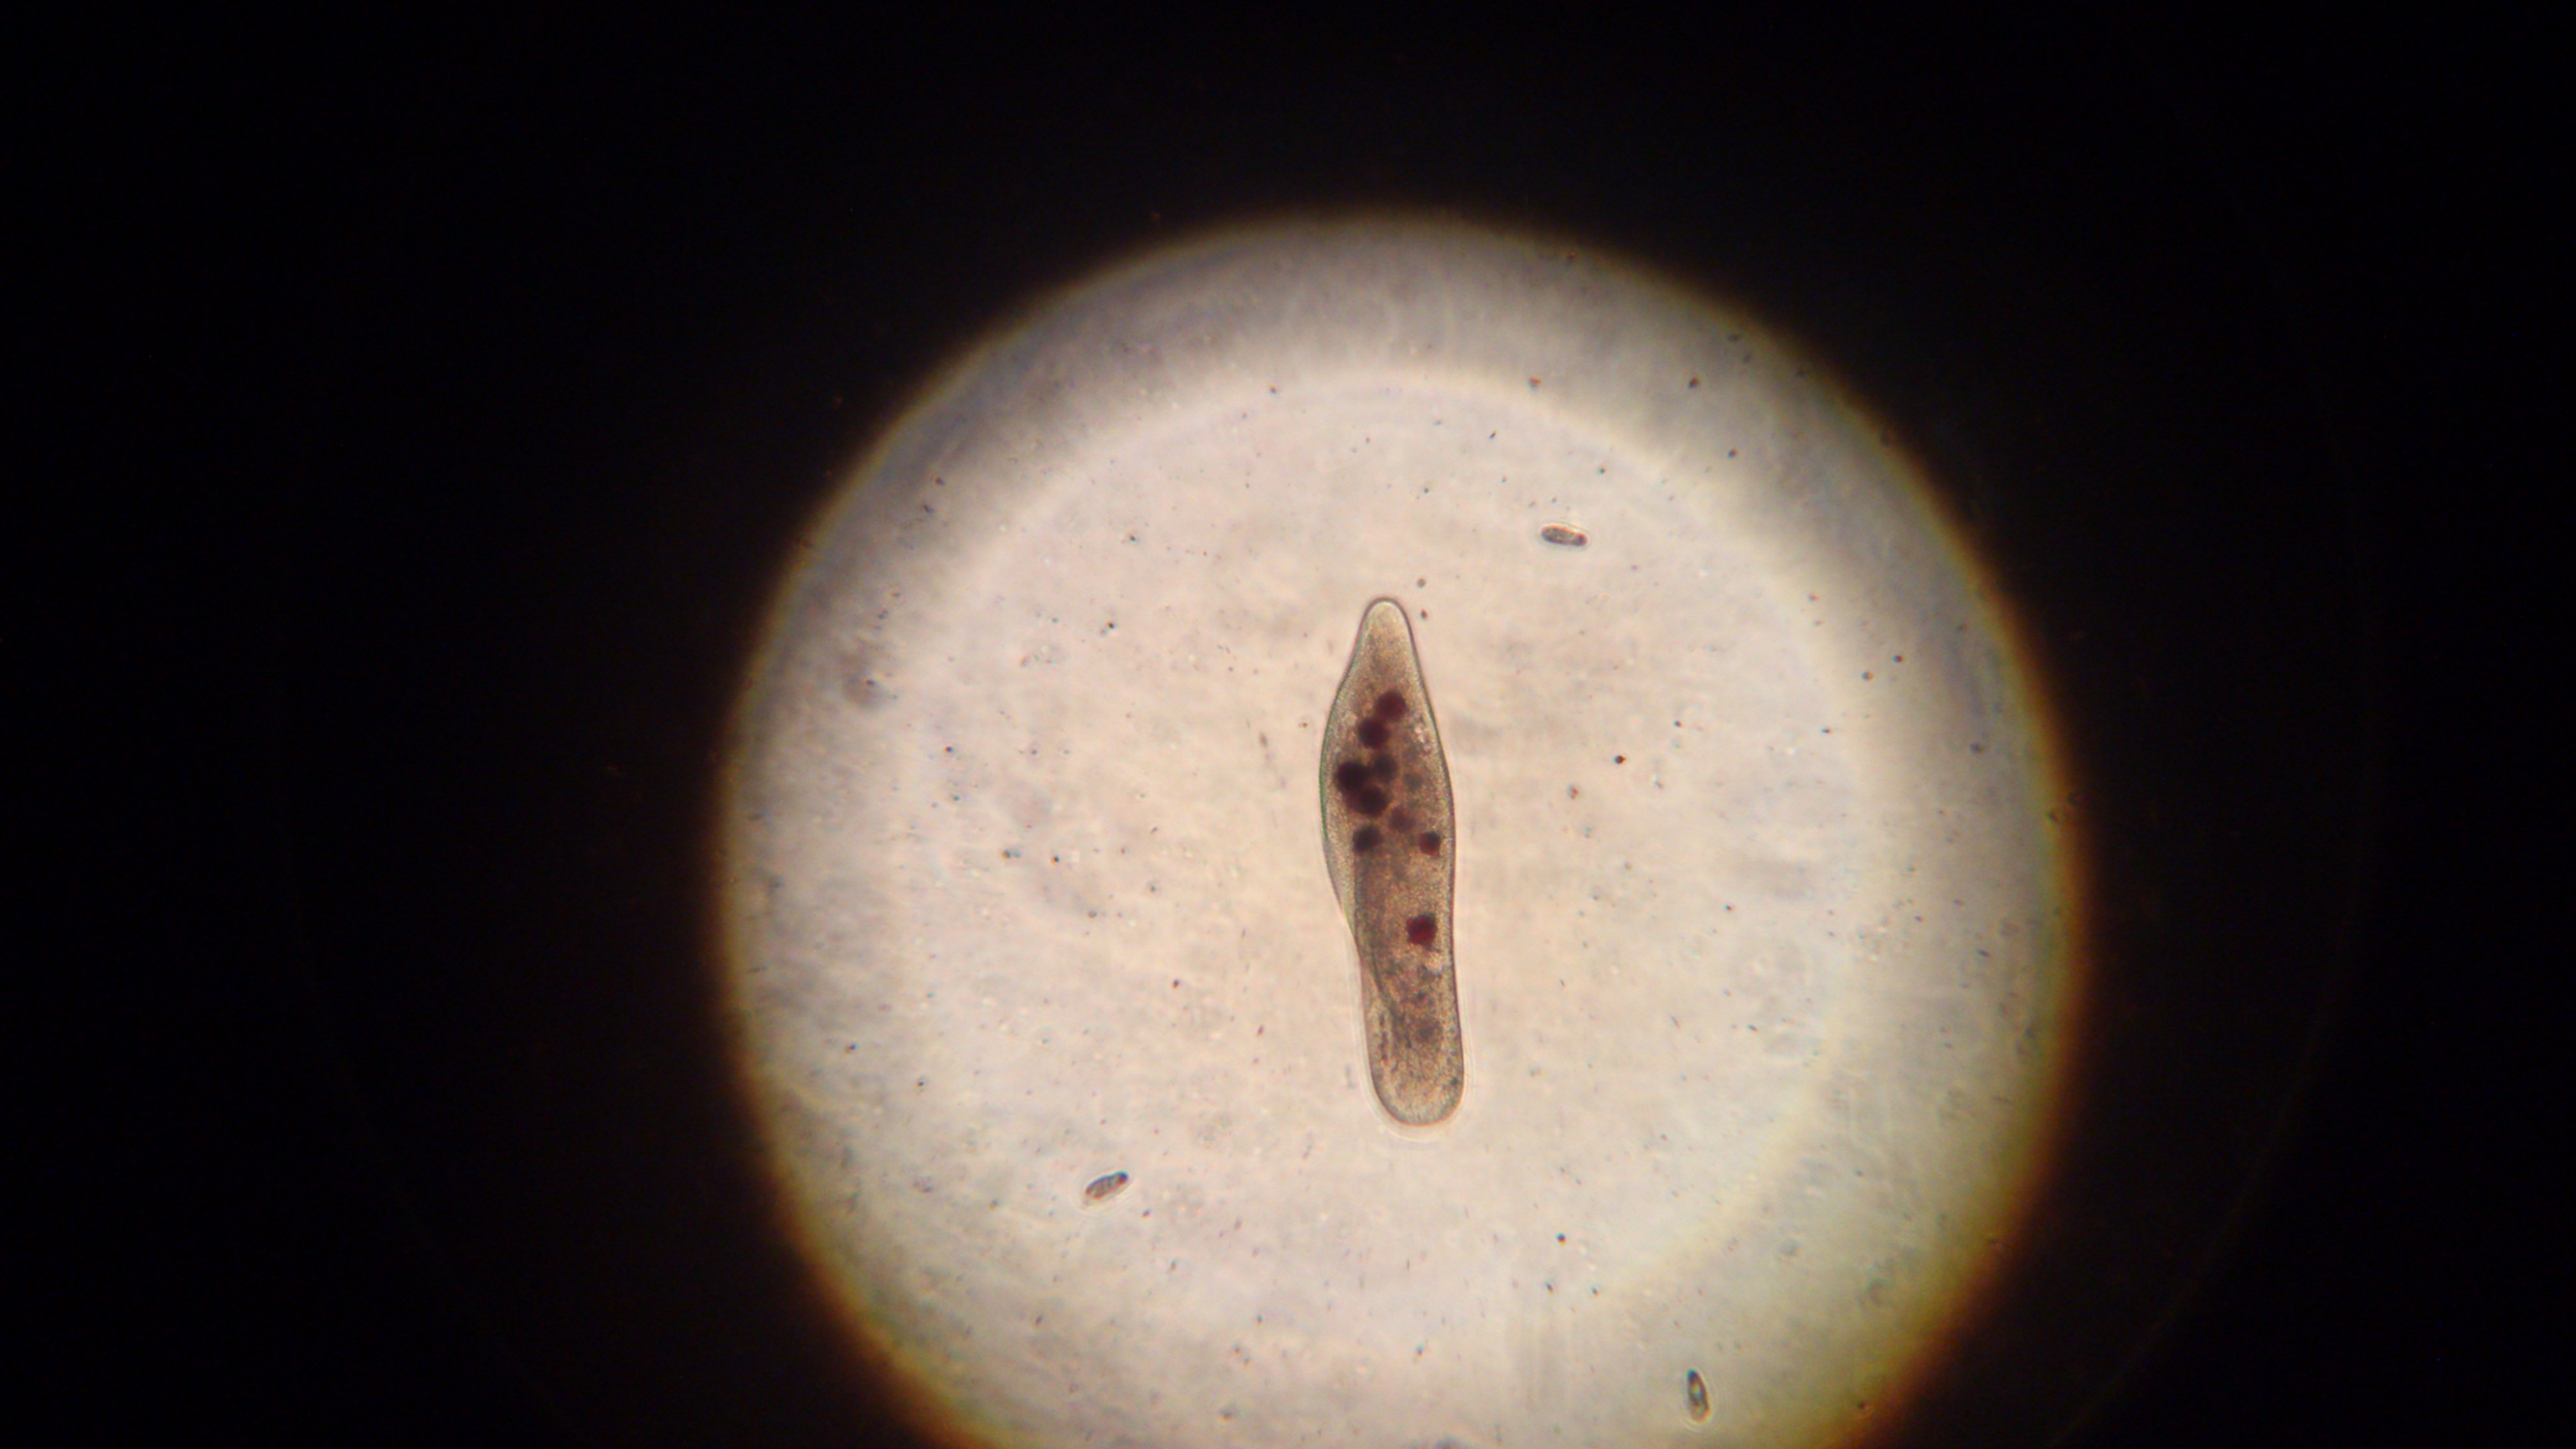
\includegraphics[width=0.5\textwidth]{fig/paramecium/DSC_1818.jpg}
    \caption{Pantoffeltierchen mit eingefärbter Hefe}
    \label{fig:paramecium}
\end{figure}\\
Die Aufnahme der Hefe kann beobachtet werden. 
Aufgrund der Bewegung der Pantoffeltierchen und des langsamen 
Verdauungsprozesses ist dieser Prozess schwierig zu beobachten. 
Jedoch können dunklere Teilchen innerhalb der Pantoffeltierchen 
beobachtet werden, welche als verdaute Hefe interpretiert wird. 
